\chapter{Solenoidal Tracker At Relativistic Heavy Ion Collider}
\label{ch:STAR}

\section{Relativistic Heavy-Ion Collider (RHIC)}
\begin{figure}[h]
	\centering
	\label{fig:RHIC-AGS}
	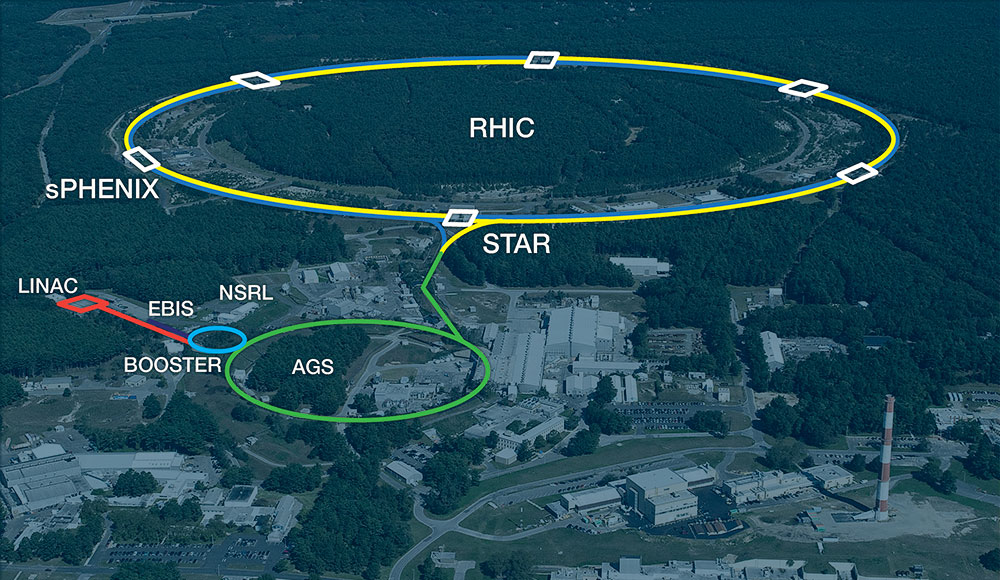
\includegraphics[width=0.6\linewidth]{figures/rhic-aerial-hr.jpg}
	\caption{An aerial view of the Relativistic Heavy Ion Collider (RHIC), showing the locations of the facilities used for accelerating different ions, and the positions of the STAR and sPHENIX detectors.}
\end{figure}

The Relativistic Heavy Ion Collider (RHIC), at Brookhaven National Laboratory (BNL), is the only collider with dedicated running for heavy ion research (the CERN Large Hadron Collider runs heavy ions for only about one month per year), and the only polarized proton collider ever built. Two concentric accelerator rings 2.4 miles in circumference containing a total of 1,740 superconducting magnets afford RHIC the capability to independently accelerate and collide ion beam species from $\rm ^1_1H (p)$ to  $\rm ^{238}_{92}U$ at energies between 3.85 GeV and 254.9 GeV per nucleon and different spin polarizations for protons (\(p\)), as shown in Fig.~\ref{fig:RHICSpecies}. These capabilities make RHIC the most flexible and capable collider in the world for transformative studies of extreme states of nuclear matter and the origin of the proton spin.

\begin{figure}[h]
	\label{fig:RHICSpecies}
	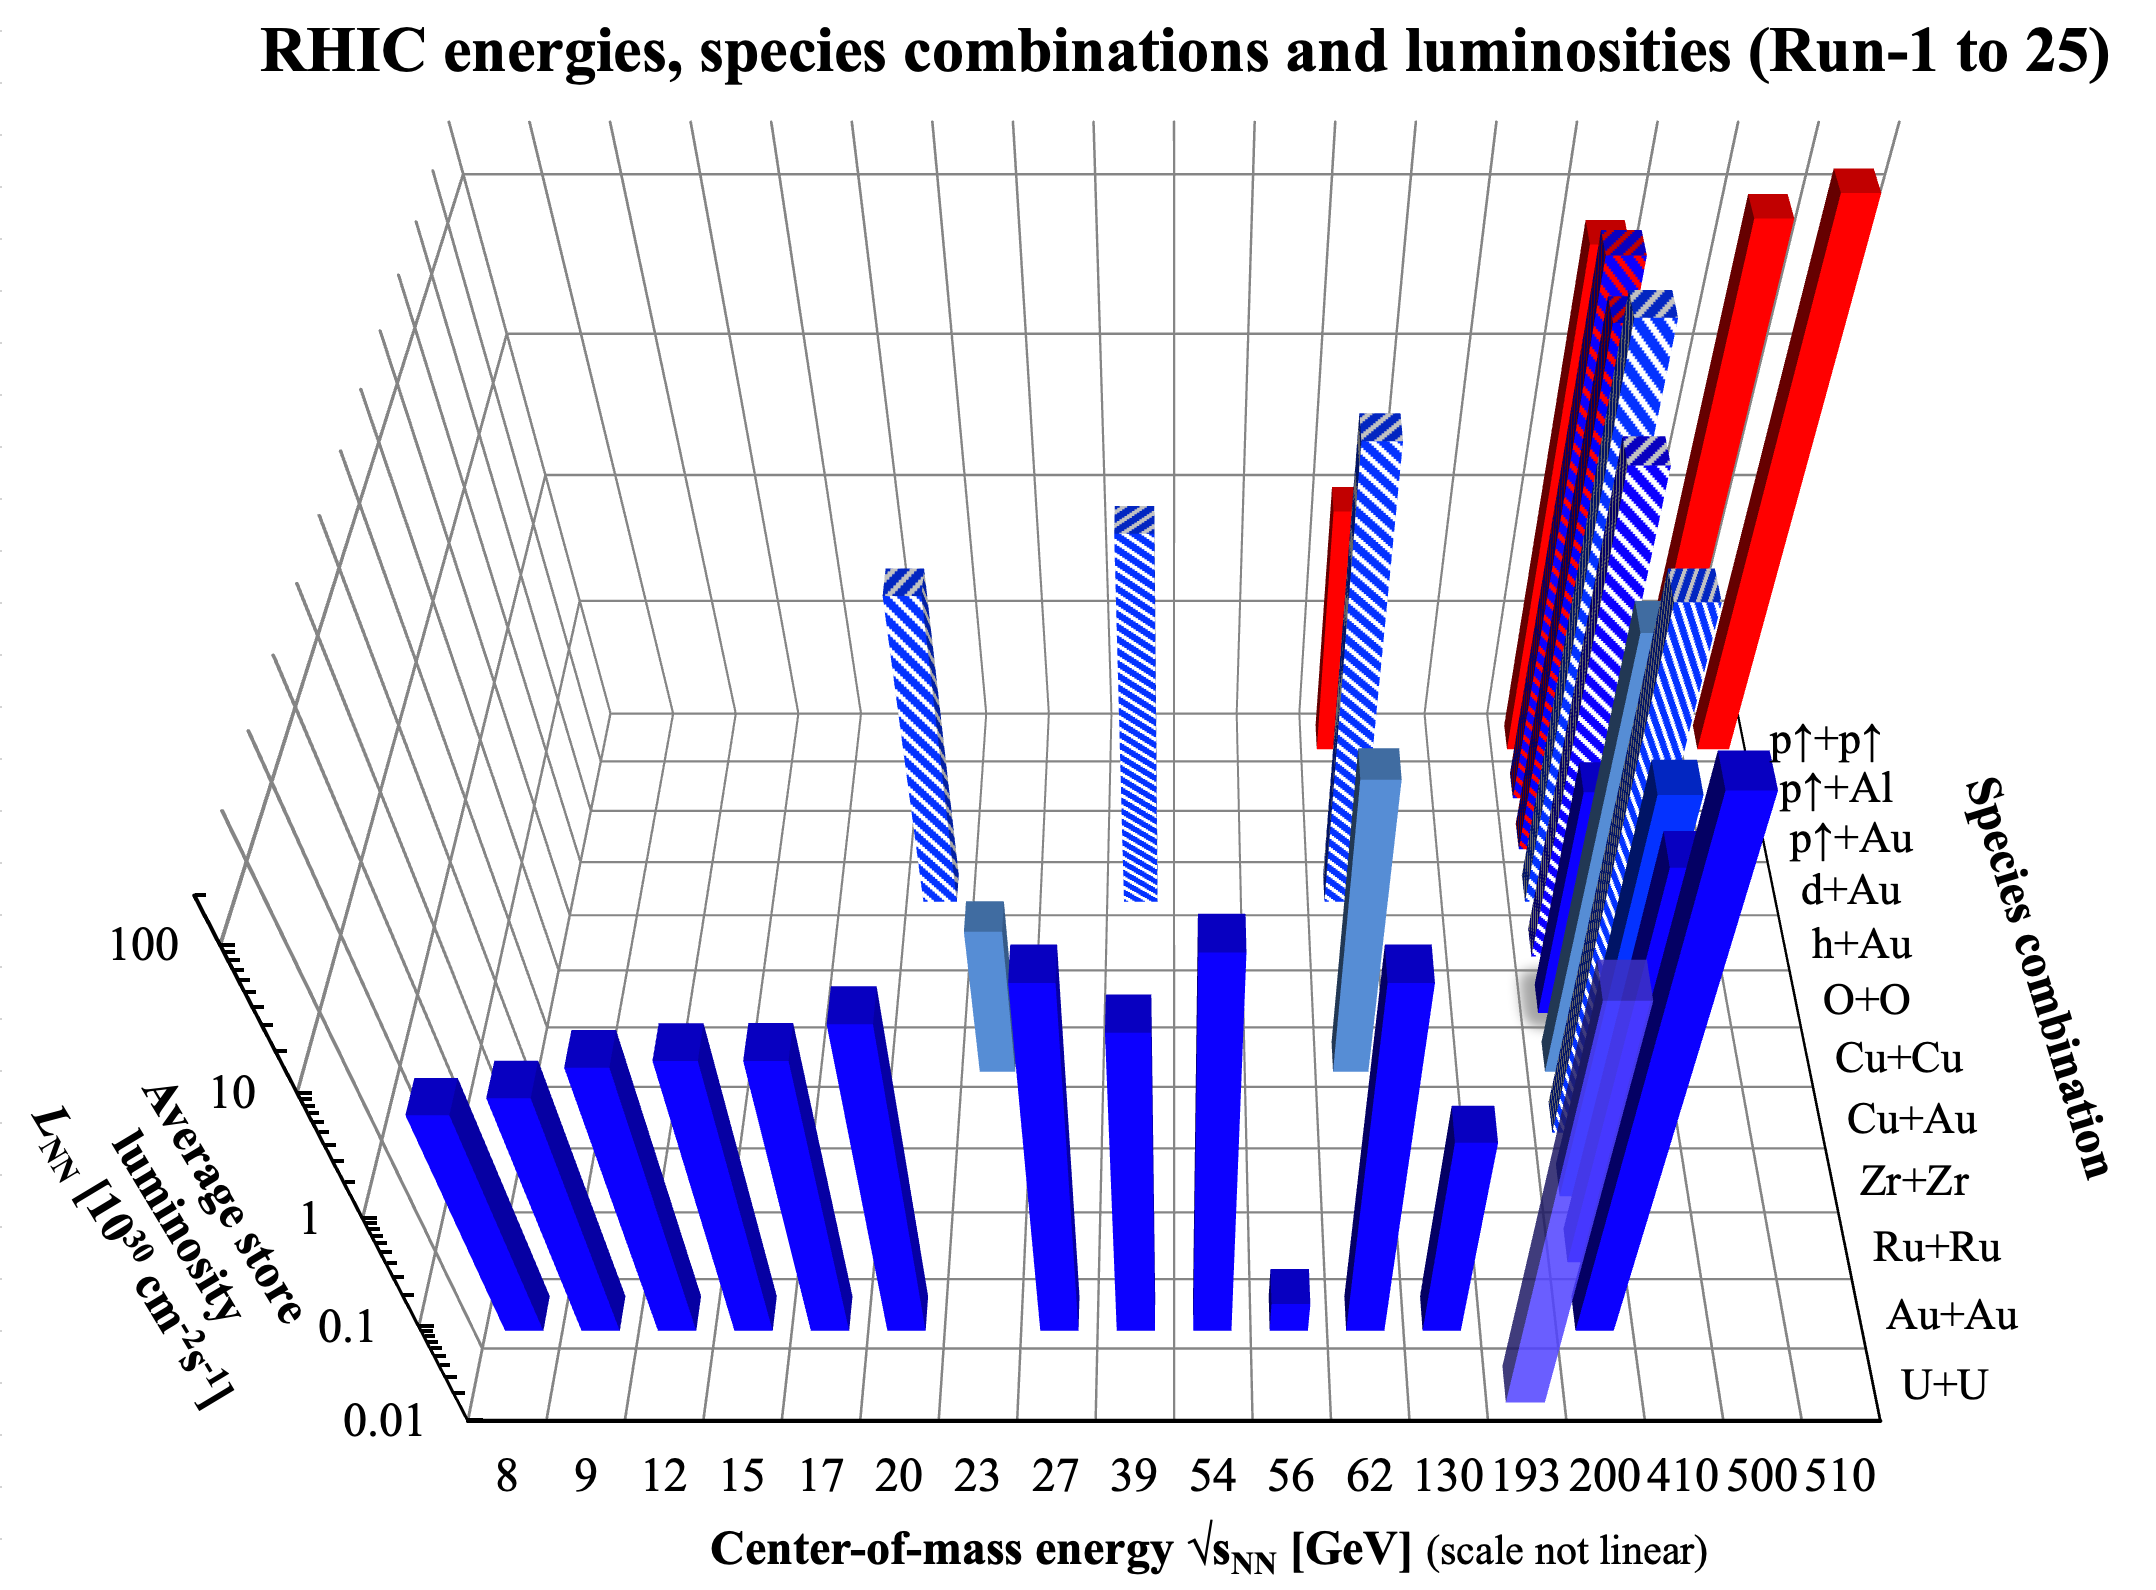
\includegraphics[width=\linewidth]{figures/RhicSpecies.png}
	\caption{Summary of RHIC energies, species combinations, and luminosities for runs between 2000 and 2026. Taken from \cite{RHICRunSummary}.}
\end{figure}
On February 6th 2026 RHIC ended operations with collisions of $\rm ^{16}_{8}O$ nuclei at \(\sqrt{s_\mathrm{NN}} = 200\)~GeV recorded by the \emph{Solenoidal Tracker At RHIC (STAR)} and \emph{sPHENIX} detectors. Over it's 25 years of active existence, it has performed \(\sim 300\)~trillion collisions of 49 unique pairs of nuclei, collected \(\sim 450\)~petabytes of data, whose analysis has led to over 650 publications. Eventually, one of RHIC’s ion storage rings will be removed and replaced with a new ring for storing accelerated electrons inside the existing accelerator tunnel, and the other major components of the RHIC accelerator complex will live on as parts of the upcoming Electron-Ion Collider (EIC).    
%\emph{strong Pioneering High Energy Nuclear Interaction eXperiment}.25 years. 

\begin{figure}[h]
	\label{fig:Final}
	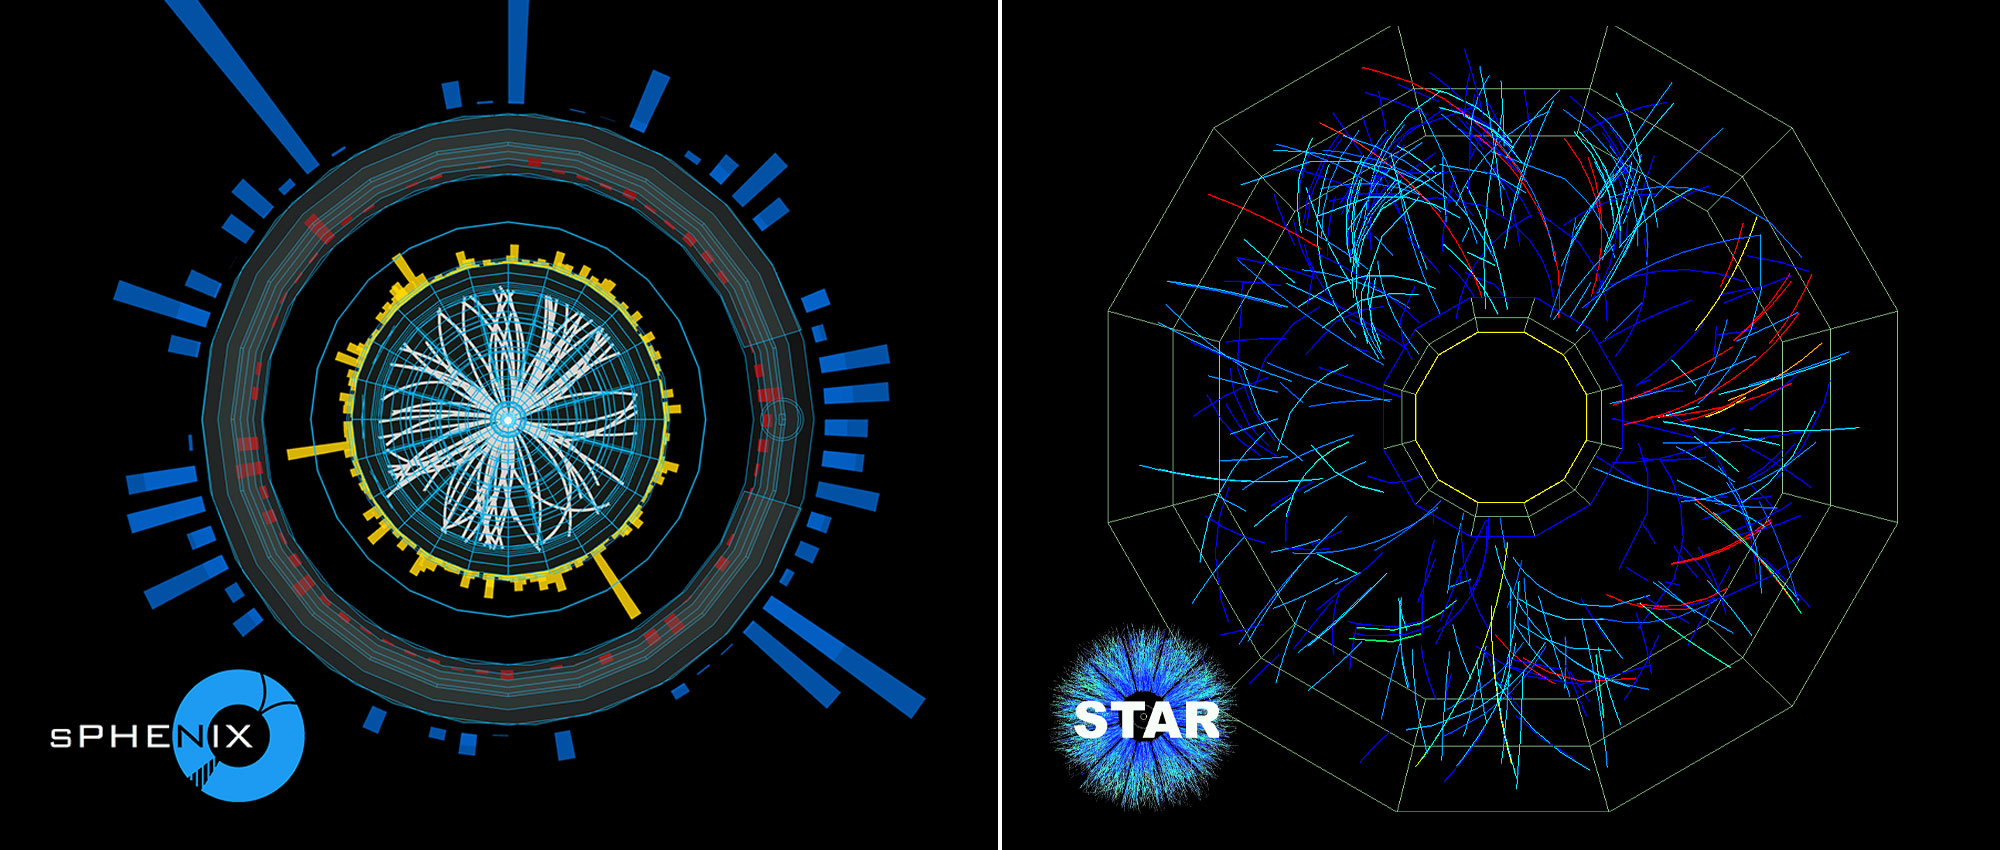
\includegraphics[width=\linewidth]{figures/sphenix-star-events-star-final-hr.jpg}
	\caption{Some of the final O+O collisions at \(\sqrt{s_\mathrm{NN}} = 200\)~GeV captured by the sPHENIX and STAR detectors at the RHIC. }
\end{figure}

\subsection{From stable matter to little bangs}
Before collisions, the nuclei have to be created first by taking the corresponding atoms and stripping off all their electrons. That process looks different for different nuclei. 
\begin{figure}[h]
	\centering
	\label{fig:AGS}
	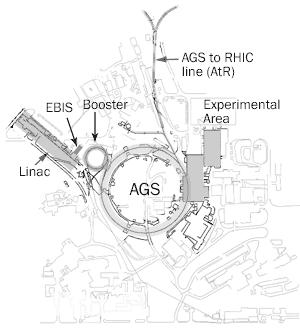
\includegraphics[width=0.5\linewidth]{figures/ags-complex}
	\caption{Schematic view of the AGS complex, showing various stages the ions go through before going into RHIC}
\end{figure}


\begin{itemize}
	\item \textbf{For protons} it is \emph{Optically Pumped Polarized \(H^-\) Ion Source (OPPIS)} fed into the \emph{Linear Accelerator (LINAC)}. The LINAC accelerates them to \(\sim 200\)~MeV and injects into the \emph{Booster Synchrotron} at which point, the two electrons are stripped away by a carbon foil. They are accelerated to upto 2.5 GeV and fed into the \emph{ Alternating Gradient Synchrotron (AGS)} which accelerates the proton beam to about 25 GeV.
	\item \textbf{For heavy-ions} like $\rm ^{197}_{79}Au$, a \emph{Laser Ion Source (LION)} extracts \(Au^+\) ions using laser ablation, which go into \emph{Electron Beam Ion Source (EBIS)} which ionizes them to \(Au^{32+}\) and accelerates them to 2 MeV per nucleon using electron beams.  Then they enter the booster synchrotron which accelerates them to about 95 MeV per nucleon. While exiting from the synchrotron, the atoms are stripped of more electrons by passing them through a stripping foil, and atoms in the $\rm Au^{77 + }$ state are fed to the AGS.  The beam's kinetic energy up to 8.86 GeV per nucleon for these Au atoms and the final two K shell electrons are stripped. 
	%Resulting beam of $\rm Au^{79 + }$ nuclei that are transported in the \emph{AtR (AGS-to-RHIC)} beampipe to the RHIC storage rings.
\end{itemize}
when the ion beam reached top speed in the AGS, it was taken down another beamline called the AGS-to-RHIC (AtR) transfer line. At the end of this line, a switching magnet sent the ion bunches down each of two beamlines to fill RHIC's two ion storage rings. Bunches directed left filled the clockwise RHIC ring (blue) while those directed right traveled counterclockwise in the second RHIC ring (yellow). In the rings, superconducting radio-frequency (RF) cavities accelerate the ion bunches to energies of 100 GeV per nucleon for heavy ions (255 GeV for protons), with four cavities operating at 28.15 MHz to generate standing waves of electric fields for the acceleration and ten 197 MHz cavities maintaining beam stability during storage. Superconducting dipole magnets with 3.5 T fields keep the beams on a circular path, while quadrupole magnets focus the ion beams. A total of 1,740 superconducting magnets are used in the two rings at RHIC, cooled by liquid Helium at $< 4.6$ K. An aerial view of the RHIC complex with the different subsystems is shown in Fig \ref{fig:RHIC-AGS}. 

There are 6 interaction regions (IR) around the RHIC complex, where the two beams cross and allow for detectors to be placed. 4 such detectors have existed during RHIC's operation: At 10 o'clock and 2 o'clock, the PHOBOS and BRAHMS experiments operated only for the first few years of RHIC (ending in 2006). At 8 o’clock, the PHENIX experiment collected data from 2000 to 2016 and was then transformed into the sPHENIX detector which began operations in 2023. STAR sits at the 6 o'clock position, and has been the only experiment running for all 25 years of RHIC's existence.

\section{The STAR detector}
STAR is designed to provide hermetic coverage around the interaction point, emphasizing precise tracking capabilities in high multiplicity environments, for its main physics mission of obtaining a fundamental understanding of the microscopic structure of QCD interactions at high energy densities.
%\begin{figure}[h]
%	\centering
%	\label{fig:STARSchematic}
%	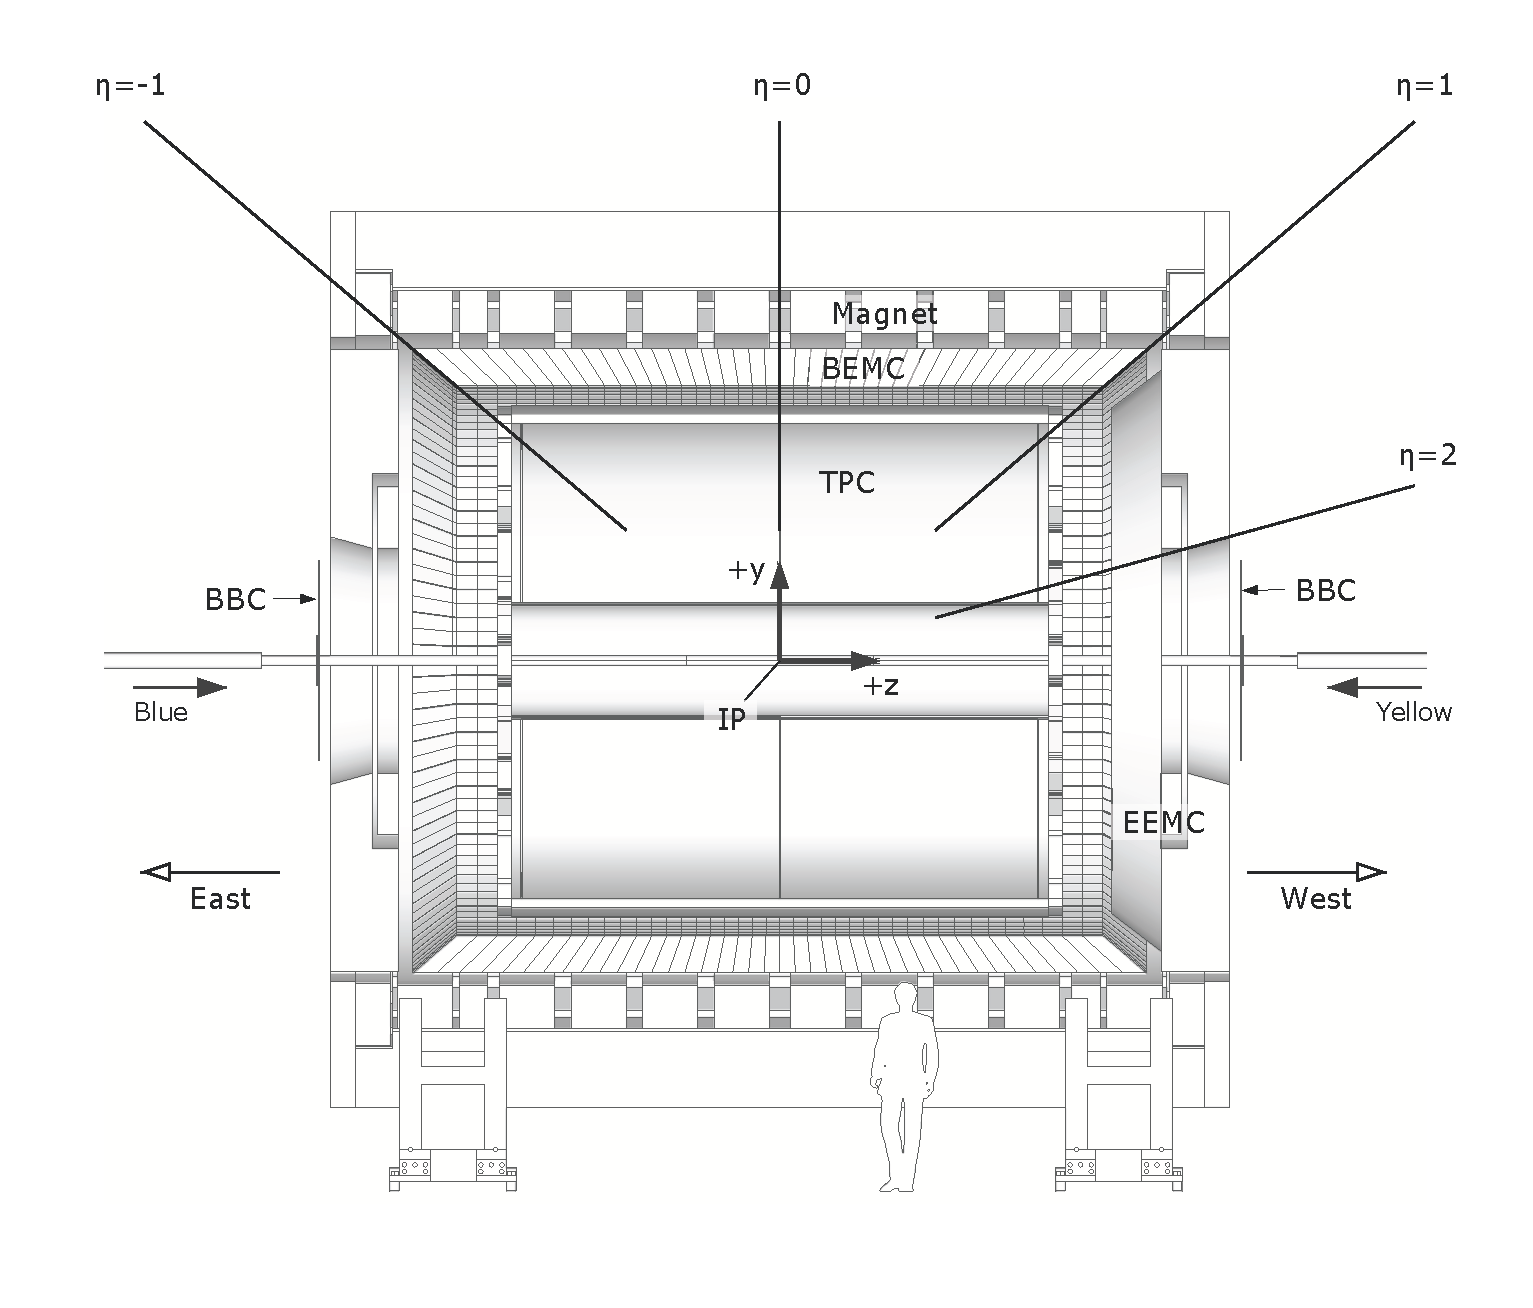
\includegraphics[width=0.8\linewidth]{figures/star_cutout.eps}
%	\caption{Illustration of the STAR Coordinate System.}
%\end{figure}

\begin{figure}[h]
	\centering
\begin{tikzpicture}
	\node[anchor=south west, inner sep=0](image) at (0,0) {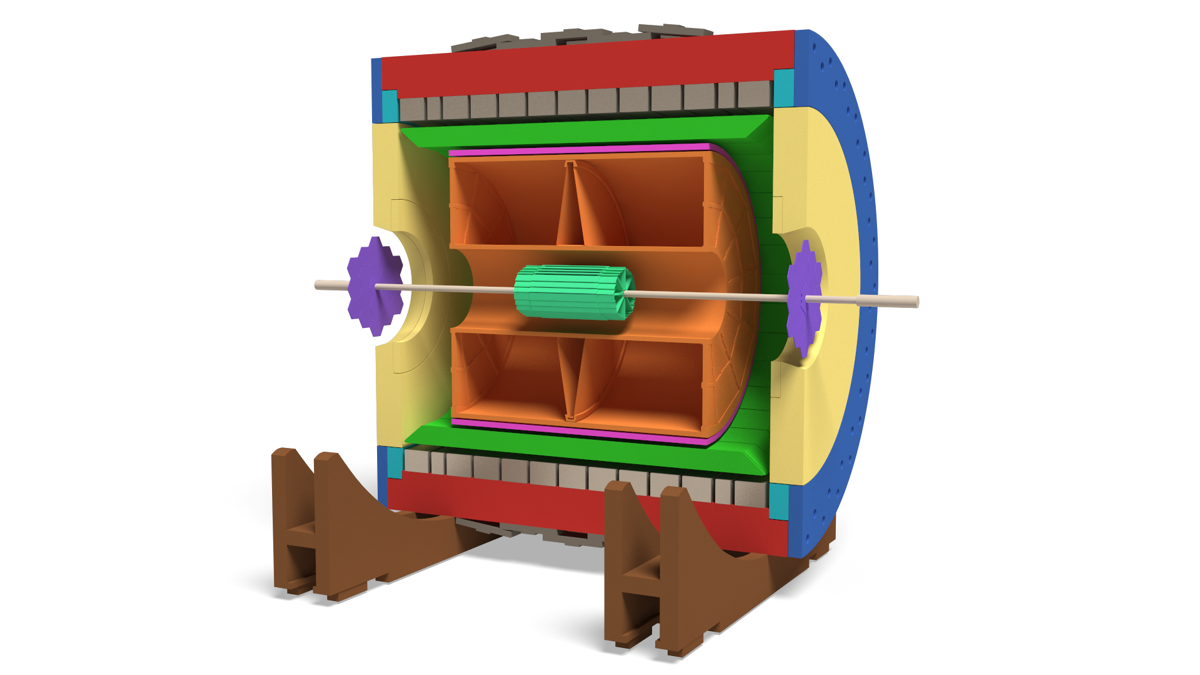
\includegraphics[width=\linewidth]{figures/STAR.png}};
	\node [anchor=west] (bemc) at (11.5,2.5) {BEMC};
	\node [anchor=west] (bbc) at (12,4.5) {BBC};
	\node [anchor=west] (tpc) at (2.5,6) {TPC};
		\node [anchor=west] (hft) at (2.5,3.5) {HFT};
		\node [anchor=west] (mag) at (2.5,8) {Solenoid};
		\node [anchor=west] (tof) at (12,7) {TOF};
				\node [anchor=west] (mtd) at (9, 9) {MTD};
	
	\begin{scope}[x={(image.south east)},y={(image.north west)}]
		\draw [-stealth, line width=1pt] (bemc) to (0.54,0.32);
				\draw [-stealth, line width=1pt] (bbc) to (0.665,0.52);
		\draw [-stealth, line width=1pt] (tpc) to (0.43,0.7);
				\draw [-stealth, line width=1pt] (hft) to (0.47,0.58);
				\draw [-stealth, line width=1pt] (mag) to (0.43,0.84);
				\draw [-stealth, line width=1pt] (tof) to (0.54,0.78);
			\draw [-stealth, line width=1pt] (mtd) to (0.54,0.96);
	\end{scope}
\end{tikzpicture}
\caption{Schematic of the STAR detector, depicting the various detector subsystems.}
\label{fig:STARDetector}
\end{figure}

It is a highly versatile, multipurpose detector with several subsystems used for triggering, tracking and identifying the particle species for charged tracks, and calorimetry. These subsystems are surrounded by a room-temperature solenoid magnet 6.2 m long and 5.26 m in diameter which generates a magnetic field of 0.5 T in the detector volume. The detector is cylindrical with full coverage in the azimuthal direction in the mid-rapidity region along with wide coverage in pseudorapidity. A schematic diagram of the STAR detector with its various detector subsystems is shown in Fig.~\ref{fig:STARDetector}. As the only experiment running continuously since the inception of RHIC, STAR has undergone major upgrades that have augmented its tracking capabilities and increased its acceptance in the forward rapidity regions. The main detectors used for this analysis are the Time Projection Chamber (TPC) and Barrel Electromagnetic Calorimeters (BEMC). 

\subsection{TPC} \label{TPC}
 Time Projection Chamber (TPC)\CITETHIS was the the primary tracking detector for STAR, providing particle identification and momentum information for charged tracks by measuring their ionization energy loss (dE/dx) inside the TPC volume\CITETHIS. As shown in Fig. \ref{fig:TPC} the TPC was a cylindrical detector 420 cm long with an outer (inner) radii of 200 (50) cm, concentric to the 0.5 T solenoid. Its acceptance covered a pseudorapidity range of $|\eta| < 1.0$, along with full azimuthal coverage. Particle momenta could be measured accurately over a range of 0.1 to 30~GeV/\(c\), and particle identification was limited between 0.1 and 1~GeV/\(c\).
\begin{figure}[h]
	\centering
	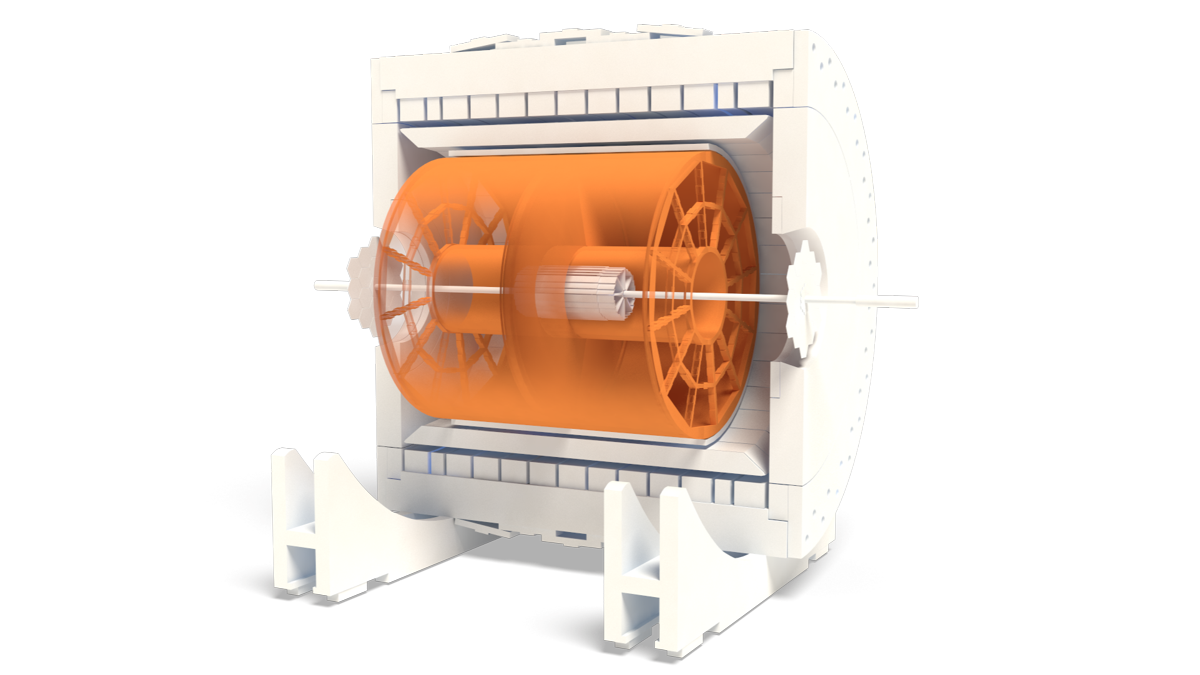
\includegraphics[width=\linewidth]{figures/TPC.png}
	\caption{The Time Projection Chamber at STAR. Taken from \cite{STARSubSystems}.}
	\label{fig:TPC}
\end{figure}
The TPC volume contained an ionizable gas mixture called P10 (10 \% methane, 90 \% argon), chosen for its high drift velocity of 5.45 $\rm cm/\mu s$ in the well-defined, uniform electric field of $\approx 135$ V/cm at STAR. 
The uniform electric field is defined between the thin conductive central membrane at z = 0 maintained at 28 kV acting as a cathode, and the two end caps each 210 cm away from the center at 0 V acting as anodes. 
The drift velocity can change over time based on atmospheric pressure fluctuations, therefore, calibrations are typically done using lasers every few hours during data-taking. 
To ensure minimal contamination by impurities like oxygen and water vapor maintained at 2 mbar above atmospheric pressure. 

\begin{figure}[h]
	\centering
	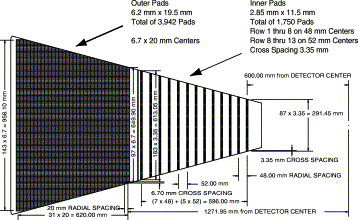
\includegraphics[width=0.7\linewidth]{figures/TPCAnode.png}
	\caption{One of the twelve sectors of the TPC. Taken from \cite{ANDERSON2003659}.}
	\label{fig:TPCAnode}
\end{figure}

The charged particles leave ionization trails were captured by Multi-Wire Proportional Counters (MWPCs)\CITETHIS with a segmented pad plane used in TPC readout.
%
As particles ionize the TPC gas, freed electrons drift toward the MWPCs under the effect of the electric field. 
%
Signal contamination was prevented using a gated grid that initially restricted electron flow, opening only if a collision is deemed significant, allowing electrons to enter the MWPCs. 
%
Positive ions generated inside the MWPC are prevented from entering the TPC’s drift volume using shield wires. 
%
The electrons passed the shield wires and were rapidly accelerated near the anode wires, creating avalanches through secondary ionization and amplifying the signal by a factor of 1,000 to 3,000. These avalanches induce signals in the surrounding pads without direct contact with the electrons. The MWPC pads detect the x-y position based on pad geometry — 3,942 pads across 32 rows in the outer sector and 1,750 pads in 13 rows in the inner sector. One such anode sector is shown in Fig. \ref{fig:TPCAnode}. The z information is then derived using the drift time and calibrated drift velocity of the electrons inside the detector volume. The typical resolution for position measurements from TPC is roughly 1 cm.
\begin{figure}
	\centering
	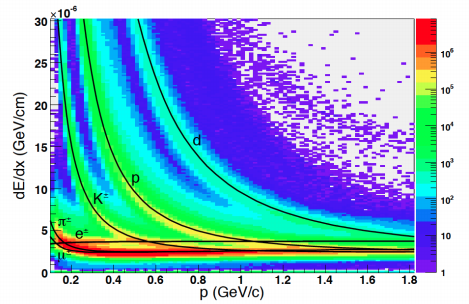
\includegraphics[width=\linewidth]{figures/dEdxVsp.png}
	\caption{The ionisation energy loss for charged particles from TPC as a function of momenta. The letters represent different particles: $\mu^{\pm}$ for muons, $e^{\pm}$ for electrons, $\pi^{\pm}$ for pions, $K^{\pm}$ for Kaons, p for protons, and d for deuterons. The solid lines are the expected value of dE/dx for the corresponding particle species from the Bichsel function \cite{BICHSEL2006154}.}
	\label{fig:dEdx}
\end{figure}

For a charged particle track, maximum of 45 hits could be recorded, which were fitted to a helix to calculate the particle momentum. Particles with momentum below 100 MeV/\(c\) curve too tightly in the magnetic field and do not reach the TPC, while those above 30 GeV/\(c\) follow nearly straight trajectories that compromise the measurement precision. For particles within these bounds, the relative momentum resolution is about 2 \%. The direction of curvature gives the charge of the track. Energy loss as a function of distance travelled, dE/dx for a track was extracted using energy loss measured by a series of pads in the TPC. Figure \ref{fig:dEdx} shows a typical plot of measured dE/dx as a function of momentum. For a given particle species with known momenta, the dE/dx curves are given by the Bichsel function \CITETHIS which are shown as solid lines in Fig. \ref{fig:dEdx}. For each particle species, the band has non-zero thickness due to the finite momentum resolution, and selection criteria based on simulations are used to assign particle ID. The particle identification from TPC is limited to low momenta tracks (about $1$ GeV/c) only beyond which the bands for different species start to overlap.

\subsection{BEMC} \label{BEMC}

The STAR Barrel Electromagnetic Calorimeter (BEMC) \cite{BEDDO2003725} designed to measure particle energies, particularly for electron and neutral particle identification.
%
BEMC was a fast detector, used as a trigger to select events containing a hard process. 
%
It also provided the neutral component of the jet energy that couldn't be reconstructed by the TPC in jet-related measurements. 
%
As shown in Fig.~\ref{fig:BEMC}, it was cylindrical detector located between the TPC and magnet coils. 
%
It covers the pseudorapidity range $|\eta| < 1$ and the full azimuth range (\(0 \leq \phi \leq 2\pi\)), matching the TPC's coverage.

\begin{figure}[h]
	\centering
	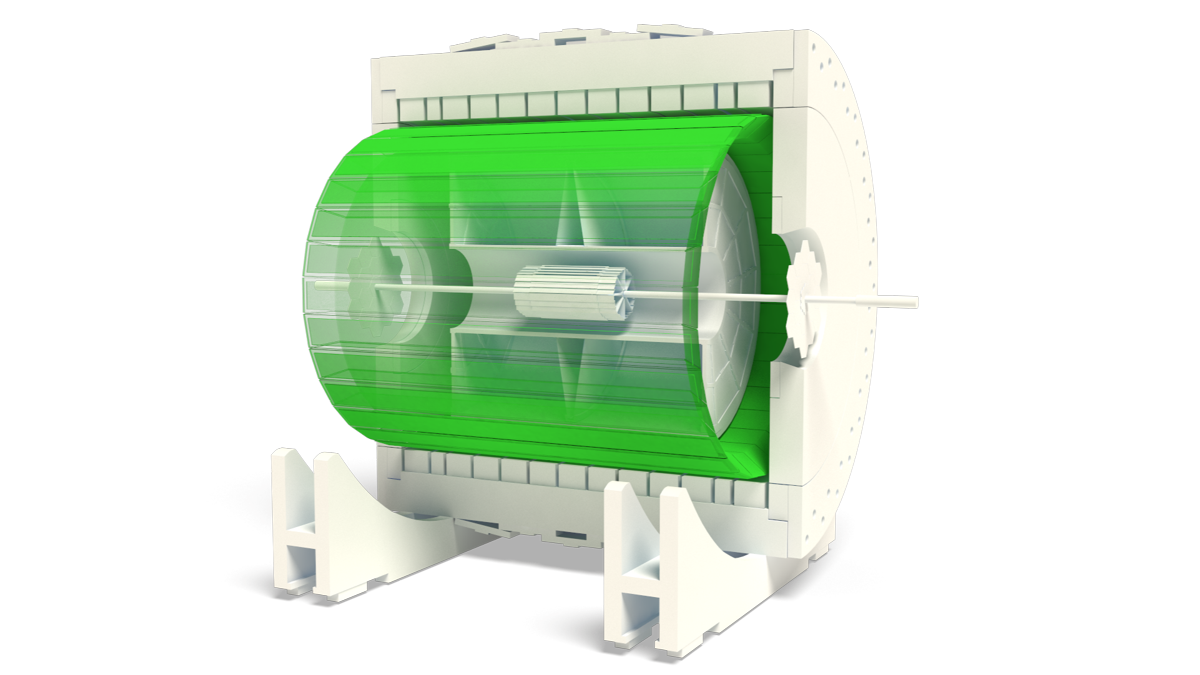
\includegraphics[width=\linewidth]{figures/BEMC.png}
	\caption{The Barrel Electromagnetic Calorimeter at STAR. Taken from \cite{STARSubSystems}.}
	\label{fig:BEMC}
\end{figure}

The inner and outer radii of the BEMC are 223.5 cm and 263 cm respectively. It consists of 120 modules, each containing 40 towers, totaling 4800 towers. Each of the towers covers a range of $\Delta \eta \times \Delta \phi = 0.05 \times 0.05$. This is approximately 10 cm × 10 cm near $\eta = 0$ and grows slightly with increasing $|\eta|$ due to their projective geometry toward the center of the detector ($z = 0$). Each BEMC tower is built with 20 alternating layers of 5-mm thick lead, which act as absorbers to initiate electromagnetic showers, and 21 layers of plastic scintillators, which detect the light produced by these showers. Together, these layers create a depth of around 20 radiation lengths ($\rm X_0$), allowing the calorimeter to capture nearly all of the energy from electromagnetic showers. This depth is enough to contain 95 \% of the energy from electrons and photons above 1 GeV. Within these layers, the Shower Maximum Detector (SMD) is located around 5-7 radiation lengths in, where the shower’s energy is most concentrated. The SMD is a gas\footnote{90 \% Argon, 10 \% $\rm CO_{2}$}-filled proportional counter and improves spatial resolution to help differentiate between the profiles of electromagnetic and hadronic showers.

The BEMC has an energy resolution that improves with particle energy, around 17\% for 1.5 GeV electrons and 10\% for 3 GeV electrons in head-on Au + Au collisions. This follows a typical calorimetric trend where energy resolution decreases as energy increases ($\sigma_{E}/E \approx 1.5 \% + 15 \% /\sqrt{E}$), providing complementarity with TPC where the resolution increases with increasing momentum ($\sigma_{p_\mathrm{T}}/p_\mathrm{T} \propto p_\mathrm{T}$).